\section{Results}\label{sec:results}

SMA-based partitioning of performance observations provides a procedural method for grouping time-correlated performance events observed during this experiment.
In the following sections, we identify regions at different timescales and apply several statistical methods over these regions to identify the breadth of performance anomalies that occur on large-scale production file systems.

\subsection{Long-term performance evolution} \label{sec:results/longterm}

\begin{figure}[t]
    \centering
    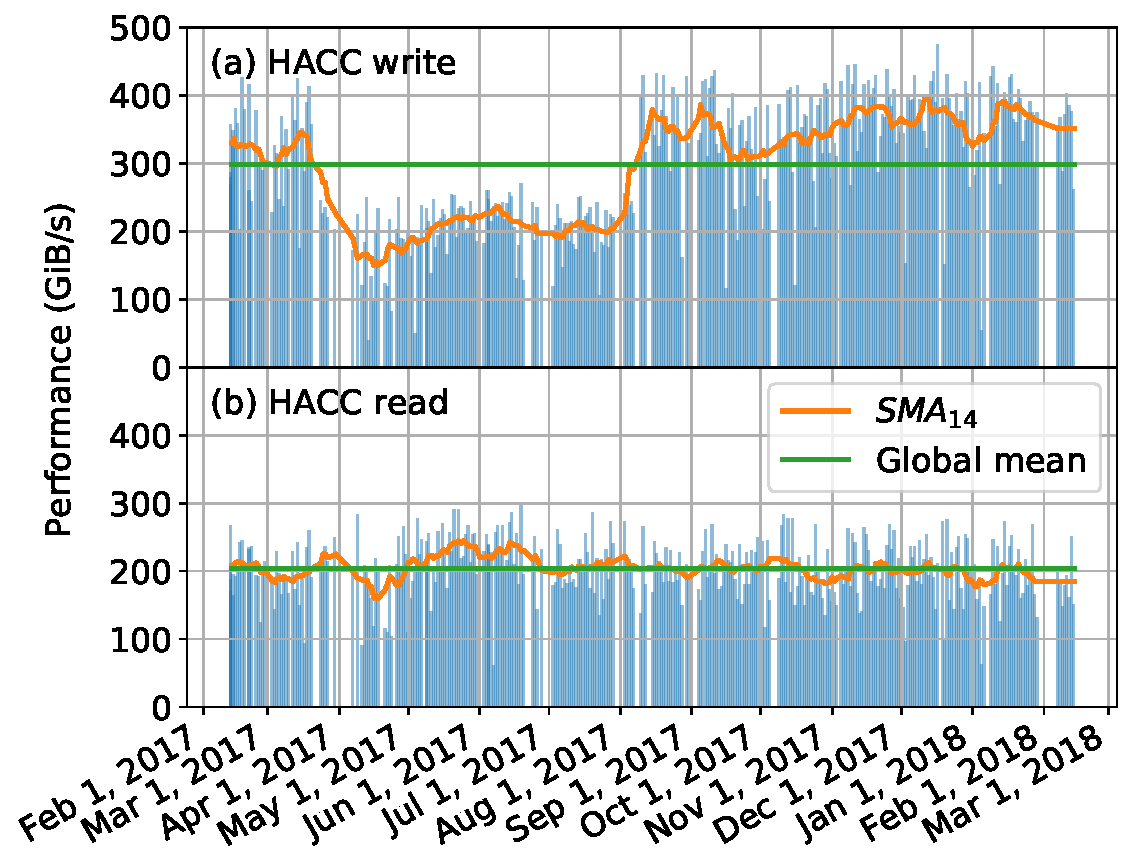
\includegraphics[width=1.0\columnwidth]{longterm-cscratch-hacc}
    \vspace{-.35in}
    \caption{Performance evolution of HACC file-per-process workload on Cori.  Red line is the overall mean (298 GiB/sec write, 204 GiB/sec read) and blue bars are raw performance measurements.}
    \label{fig:timeseries-baseline}
%   \vspace{-.3in}
% UP01 to UP03 upgrade, UP03 to UP04
\end{figure}

The horizontal bands in Figures \ref{fig:summary-heatmap} and \ref{fig:regions-heatmap}b identify long periods of reduced performance for the file-per-process write workloads as dark horizontal bands between April and August.
Because this region occurred over a period of months, we choose a ${w_{short}} = 28$ days to minimize the effects of high-frequency transients and ${w_{long}} \rightarrow \infty$ to identify performance regions that are abnormal relative to the global mean performance.  The resulting SMAs for the HACC write workload on Cori are shown in Figure \ref{fig:timeseries-baseline}a.

The intercepts between $\textup{SMA}_{28}$ and $\textup{SMA}_{\infty}$ visibly distinguish the extent of the long-term performance depression that occurred between April and August for the HACC write workload.
This performance region defining this performance depression lasted for 139 days, and no other performance regions were identified for this workload.
In stark contrast, the performance of HACC read workload (Figure \ref{fig:timeseries-baseline}b) was unaffected during this time; the longest performance region identified was 59 days long and exhibited abnormally \emph{high} performance.
Incidentally, this abnormally high performance occurred between May 7 and July 4--a time when the HACC write performance was also experiencing high performance \emph{relative to its long-term performance depression.}

These data demonstrate that the nominal peak performance of specific applications' I/O can vary over the service life of a storage system and its dependent components.
Furthermore, the difference between the read and write motifs in Figure \ref{fig:timeseries-baseline} indicates that not all workloads are affected by long-term variation equally. 
In this case of HACC on Cori, write performance was adversely for a period of months while read performance of the same I/O pattern was completely unaffected.

In combination with expert knowledge, the root cause for the long-term performance depression in the HACC write workload was retrospectively identified using the boundaries of the 139-day performance region.
The intersection between $\textup{SMA}_{28}$ and $\textup{SMA}_\infty$ in Figure \ref{fig:timeseries-baseline} occurs at March 24 and August 10, and comparing these dates to the service history of Cori revealed that operating system upgrades occurred on exactly those dates--March 24 and August 10.
The Lustre client versions were updated on those two dates, and the appearance and subsequent disappearance of the anomalous behavior was attributed to a bug in the client software.

Finally, our choice of averaging $\textup{SMA}_{short}$ over ${-0.5w_{short} <= t < +0.5w_{short}}$ makes it insensitive to choice of $w_{short}$.
For this dataset, reducing $\textup{SMA}_{short}$ from $\textup{w}_{28}$ to $\textup{w}_{7}$ resulted in no change to the dates bounding the 139-day performance region.
The only effect was the identification of a larger number of short performance regions with widths on the order of seven days.





\subsection{Transitions between performance regions} \label{sec:results/transitions}

\begin{figure}
    \centering
    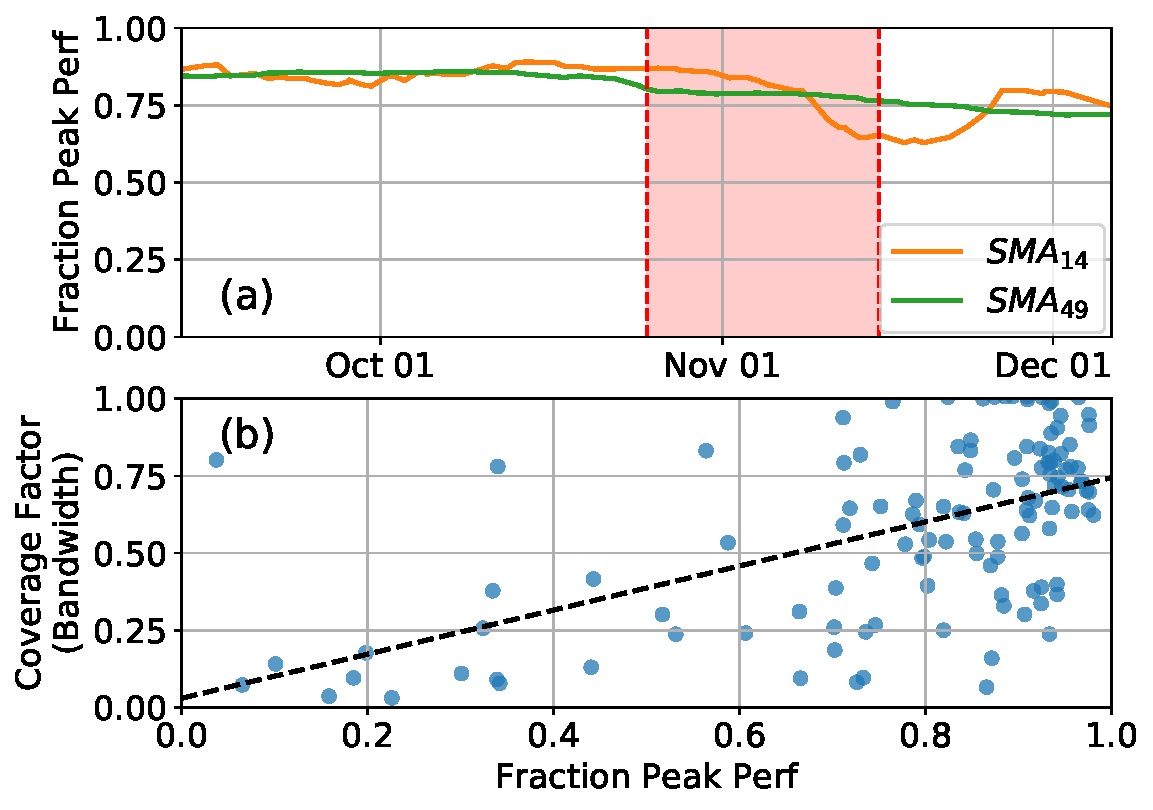
\includegraphics[width=1.0\columnwidth]{mira-correlation-region}
    \vspace{-.35in}
    \caption{Correlation between performance and $CF_{bw}$ in a transition between performance regions on Mira. (a) shows a region automatically detected using the centroid method, and (b) shows the correlation between performance and $CF_{bw}$ in that region.  Correlation coefficient is $0.565$ and p-value is ${1.48 \times 10^{-11}}$; dashed line in (b) is a linear fit with slope $0.714$ drawn for visual aid.}
    \label{fig:mira-correlation-region}
%   \vspace{-.3in}
% UP01 to UP03 upgrade, UP03 to UP04
\end{figure}

Long-term behavior has very low frequency by definition, so analyzing the causes of a few long-term performance depressions by hand (as was done in Section \ref{sec:results/longterm}) is not unreasonable.
With smaller values of $w_{long}$, though, this method identifies an increasing number of performance regions, and characterizing the factors that contribute to these long-term performance depressions using automated statistical techniques becomes imperative.

Performance can be effectively correlated with other metrics collected during I/O-intensive jobs if

\begin{enumerate}[leftmargin=*]
\item a sufficient number of similar jobs ran during a temporal region of interest to establish statistical confidence, and \label{sec:results/transitions/criterion1}
\item sufficient variation in performance is observed in the neighboring jobs to establish compelling correlation coefficients \label{sec:results/transitions/criterion2}
\end{enumerate}

To identify performance regions of sufficient width to satisfy (\ref{sec:results/transitions/criterion1}), we apply SMAs with judiciously chosen values of $w_{short}$ and $w_{long}$ to establish regions that capture enough measurements to calculate correlations with high confidence.
We also discard all intersection points that would terminate a performance region containing fewer than seven observations, effectively aggregating multiple short performance regions into larger ones.
To satisfy (\ref{sec:results/transitions/criterion2}) and capture regions that exhibit a broad range of performance measurements, we convert pairs of performance regions into \emph{transition regions} as defined in Section \ref{sec:features}.
We then discard transition regions whose $\textup{SMA}_{short}$ exhibit minimal change between their first and last value in the region.  For each transition region bounded by times $t_0$ and $t_f$, we then discard those regions where

\begin{equation}
abs \left (
\frac
	{ \textup{SMA}_{short}(t_0) - \textup{SMA}_{short}(t_f) }
	{\textup{SMA}_{short}(t_f)}
\right ) < C
\end{equation}

and $C$ is a cutoff threshold typically between 0.15 and 0.40 whose optimal value is a function of $w_{short}$, $w_{long}$, and how variable the storage system performance tends to be over long periods of time.
Given a well-chosen $C$, the result set of transition regions satisfy both the (\ref{sec:results/transitions/criterion1}) sampling criterion and (\ref{sec:results/transitions/criterion2}) diversity criterion.

To demonstrate the utility of this approach, we apply it to the entirety of performance observations across all benchmarks run on Mira.
Using $w_{short} = 14$ and $w_{long}$ = 48 with a cutoff $C = 0.15$ results in only two transition regions are identified for the entire year, consistent with the relatively stable performance of Mira shown in Figure \ref{fig:summary-heatmap}.
For each transition region, we then calculate the Pearson correlation coefficient between the fraction peak performance observations and the other telemetric data associated with each job as described in Section \ref{sec:methods/tokio}.

Discarding all correlations with low confidence ($\textup{p-value} > {1.0 \times 10^{-5}}$), only one of the two regions (shown in Figure \ref{fig:mira-correlation-region}a) exhibited significant correlation between performance and any other metrics.
Furthermore, the bandwidth coverage factor was the only metric that showed moderate correlation (${R = 0.565}$) with high confidence ($\textup{p-value} < 1.4 \times 10^{-11}$), as shown in Figure \ref{fig:mira-correlation-region}b.
While we cannot determine causation from this correlation, we can confidently state that this analysis identified a long-term performance transition between October 13 and November 15 that was strongly correlated with bandwidth contention.
The fact that this performance degradation was observed across all I/O motifs distinguishes it from the case discussed in section \ref{sec:results/longterm} and further indicates a system-wide loss of performance.
Given that sustained performance degradation was not detected at any other time during the year, the contentious activity that coincided with this performance depression on Mira was likely not caused by routine job traffic and may have been related to year-end activity on the system.







\subsection{Shorter-term behavior} \label{sec:results/shortterm}

\begin{figure}[t]
    \centering
    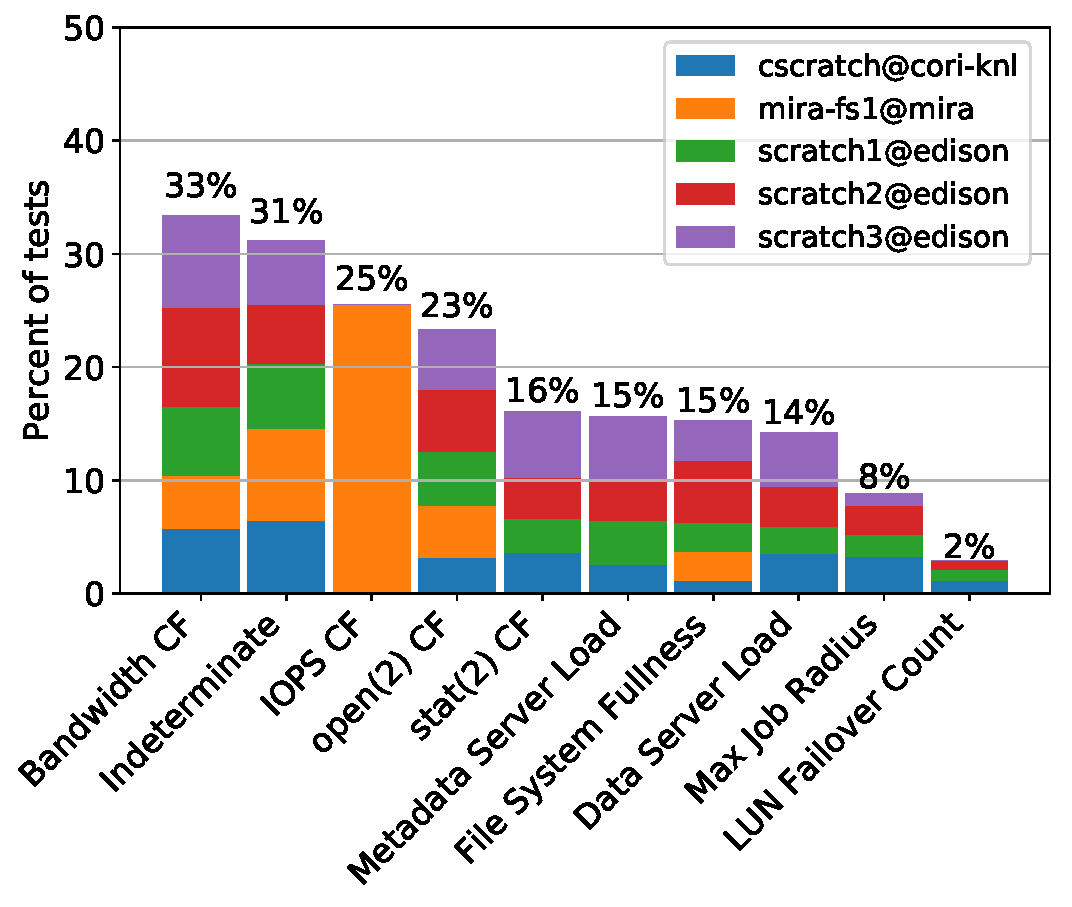
\includegraphics[width=1.0\columnwidth]{contributors-bad-by-system}
    \vspace{-.35in}
    \caption{Metrics that correlated with poor I/O performance across all file systems and benchmarks tested.  "CF" refers to coverage factor as defined earlier; "Indeterminate" are those jobs where no metrics could be classified as contributors.
    \TODO{Shall we add some explanation for coverage factor as the reviewers may not be familiar with UMAMI? --Teng}}
    \label{fig:contributors-bad-by-system}
%   \vspace{-.3in}
% UP01 to UP03 upgrade, UP03 to UP04
\end{figure}

During this experiment, we often observed the case where application performance was severely degraded for one and only one day in an otherwise unremarkable performance region.  
The lack of a gradual transition of performance around these bad days results in a low-diversity set of observations that limits the confidence of correlation-based classification.

To automatically classify the factors contributing to these isolated days of transient performance loss, we first separate performance observations based on three criteria: the test application, whether the application was reading or writing, and the file system on which the test was run.
Each resulting set of \{app, r/w, system\} was then partitioned using the interception points of $\textup{SMA}_{7}$ and $\textup{SMA}_{28}$ and resulted in between 16 and 27 performance regions.

\TODO{A few sentences answering why 16 and 27 regions are generated may be helpful. May also replace 40 by 5$\times$4$\times$2 for easier understanding -Teng}

\begin{enumerate}[leftmargin=*]
\item The lowest performance measurement of that region is identified as a Job of Interest
\item TOKIO's UMAMI analysis is performed where metrics that speak to application-side performance, file system load, file system health, system batch scheduler load, and system topology are all combined into a single holistic description of each job's I/O performance
\item The value of each metric measured during the Job of Interest is compared to the statistical distribution of those metrics across all other jobs in the performance region.  All metrics whose values were at their worst at the same time the Job of Interest was running are flagged as potential contributors to the poor performance of the job of interest.
\end{enumerate}

The result of this analysis is zero or more metrics being flagged as potential contributors to poor performance within each performance region for each application, file system, and read/write mode.

Aggregating all of the performance regions' poor-performance contributors yields a broad overview of the metrics that most commonly coincide with poor performance across all of the test systems.
This distribution, shown in Figure \ref{fig:contributors-bad-by-system}, reveals that abnormally high bandwidth contention was found to coincide with abnormally poor performance most frequently.

\TODO{Define the metrics in Fig \ref{fig:contributors-bad-by-system}}

\TODO{Somewhere, maybe not here, revisit findings from PDSW paper and see if
they still make sense in year long context?}